% !TEX encoding = UTF-8 Unicode
% !TEX root = ../Saunkin.tex


\chapter{Methodology} \label{c2:methodology}

The previous chapter presented an overview of existing systems and approaches to citation analysis.
These approaches rely on structured representations of publications and their relationships, typically in the form of citation networks.
This chapter introduces a data model representing publications and authors, and then proposes a methodology for distinguishing between self-citations and external citations.


\section{Data model} \label{sec:data-model}

The goal of the model proposed in this section is to define the minimum structure required for identifying and classifying citations.

We identify two entities in the data of this system:

\begin{description}

    \item [Author] represents a researcher associated with one or more scientific papers.
    Each author is identified by the name under which the paper is published.

    \item[Paper] represents a scientific publication.
    Each paper is described by a set of properties, forming a natural key: title, year of publication, and list of authors.

\end{description}

Two relationships are identified between the entities:

\begin{description}

    \item[Authorship] relationship connects authors and papers.
    A paper has one or more authors, and an author may write one or more papers (many-to-many).

    \item[Citation] represents a reference from one paper to another.
    A paper may cite and be cited by multiple other papers (many-to-many).

\end{description}

\enote{I have no way to put this figure under the Citation definition in the PDF - this figure keeps appearing in the middle of the page}

Figure~\ref{fig:er-model} presents the data model used in this work and described above.

\begin{figure}
    \centering
    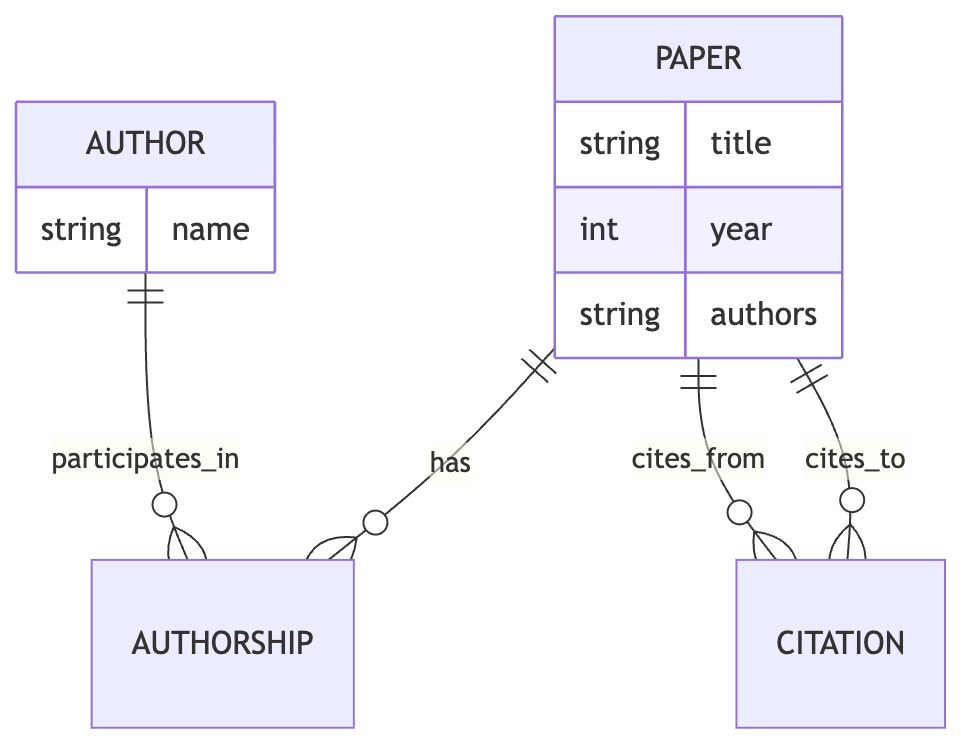
\includegraphics[width=10cm]{include/fig-data-model-er-diagram}
    \caption{Conceptual ER model for citation analysis}
    \label{fig:er-model}
\end{figure}

In addition to the authorship relationship, the author list (as it appears in the publication) is also retained as a property of the paper.
This reflects the way publications are usually identified, where author names form part of the citation string.
While the \emph{authorship} provides the structural relationship between authors and papers, the \emph{authors} attribute is used for identification.


\section{Classification of citations} \label{sec:citation-classification}

Based on the data model defined in the previous section, each citation can be classified by the relationship between the authors of the citing and cited papers.
The classification depends on whether the two papers share any authors.

A citation is classified as a \emph{self-citation} if at least one author appears in both the citing and the cited paper.
This definition is widely adopted in related studies, where self-citations are identified based on authorship overlap between publications~\cite{Glnzel2003BIBLIOMETRICSAA, Fowler2007}.
If the citing and cited papers do not share any authors, the citation is classified as an \emph{external citation}.

In addition to the basic distinction, self-citations can be further refined, to distinguish between citations made directly by the same author and those less strict, that arise naturally through citation of co-authored papers.
A citation is classified as a \emph{direct self-citation} of the author under analysis, if the author appears in both the citing and the cited paper.
A citation is classified as a \emph{co-author self-citation}, if the two papers share at least one author, but the author under analysis does not appear in the citing paper.

\section{Aggregation and Processing Pipeline} \label{sec:aggregation-pipeline}

The classification of citations is used to analyze citation behavior at the level of an individual author.

For a given author \(a\), the goal is to evaluate the citations received by the papers authored by \(a\), and to distinguish between different types of citations.

The process consists of the following steps:

\begin{itemize}
    \item All papers authored by \(a\) are identified.
    \item For each paper \(P_i\), all incoming citations are collected.
    \item These citations are classified according to the definitions provided in Section~\ref{sec:citation-classification}.
\end{itemize}

Following this process, the following counts can be evaluated for the author \(a\):

\begin{itemize}
    \item Total number of citations received by all papers authored by \(a\)
    \item Number of self-citations
    \item Breakdown into direct and co-author self-citations
    \item Number of external citations
\end{itemize}

Optionally, numbers produced by this pipeline can be evaluated against known metrics (e.g. Fi-score).

\section{Assumptions and limitations} \label{sec:assumption-and-limitations}

The methodology presented in this chapter assumes the availability of structured data describing publications, authors, and citation relationships.
In practice, the acquisition and quality of such data introduce several constraints.

\begin{itemize}
    \item Access to citation data is provided through external systems, typically imposing rate limits, which restricts the volume of data that can be retrieved within a time frame.
    \item Different sources provide inconsistent coverage of publications and metadata, which affects the quality of the citation graph.
    \item Identification of authors across publications is not uniquely standardized.
    Difference in naming and identifiers leads to ambiguity when determining whether publications refer to the same author.
\end{itemize}

These factors do not affect the formal definitions introduced in this chapter, but they influence the practical application of the methodology and are considered in the implementation described in the following chapter.
